%% Figure 2 (fig:workflow) — CAMELS-RU production workflow schematic.
%% Standalone TikZ source; copernicus.cls loads the times font, matched here.
%% Build (from repo root):
%%   pdflatex -output-directory=paper/figures_src paper/figures_src/fig_workflow.tex
%%   cp -p paper/figures_src/fig_workflow.pdf paper/images/fig_workflow.pdf
%%   cp -p paper/figures_src/fig_workflow.pdf paper/overleaf/images/fig_workflow.pdf
\documentclass[border=2mm]{standalone}
\usepackage{times}
\usepackage{tikz}
\usetikzlibrary{positioning,arrows.meta}

\begin{document}
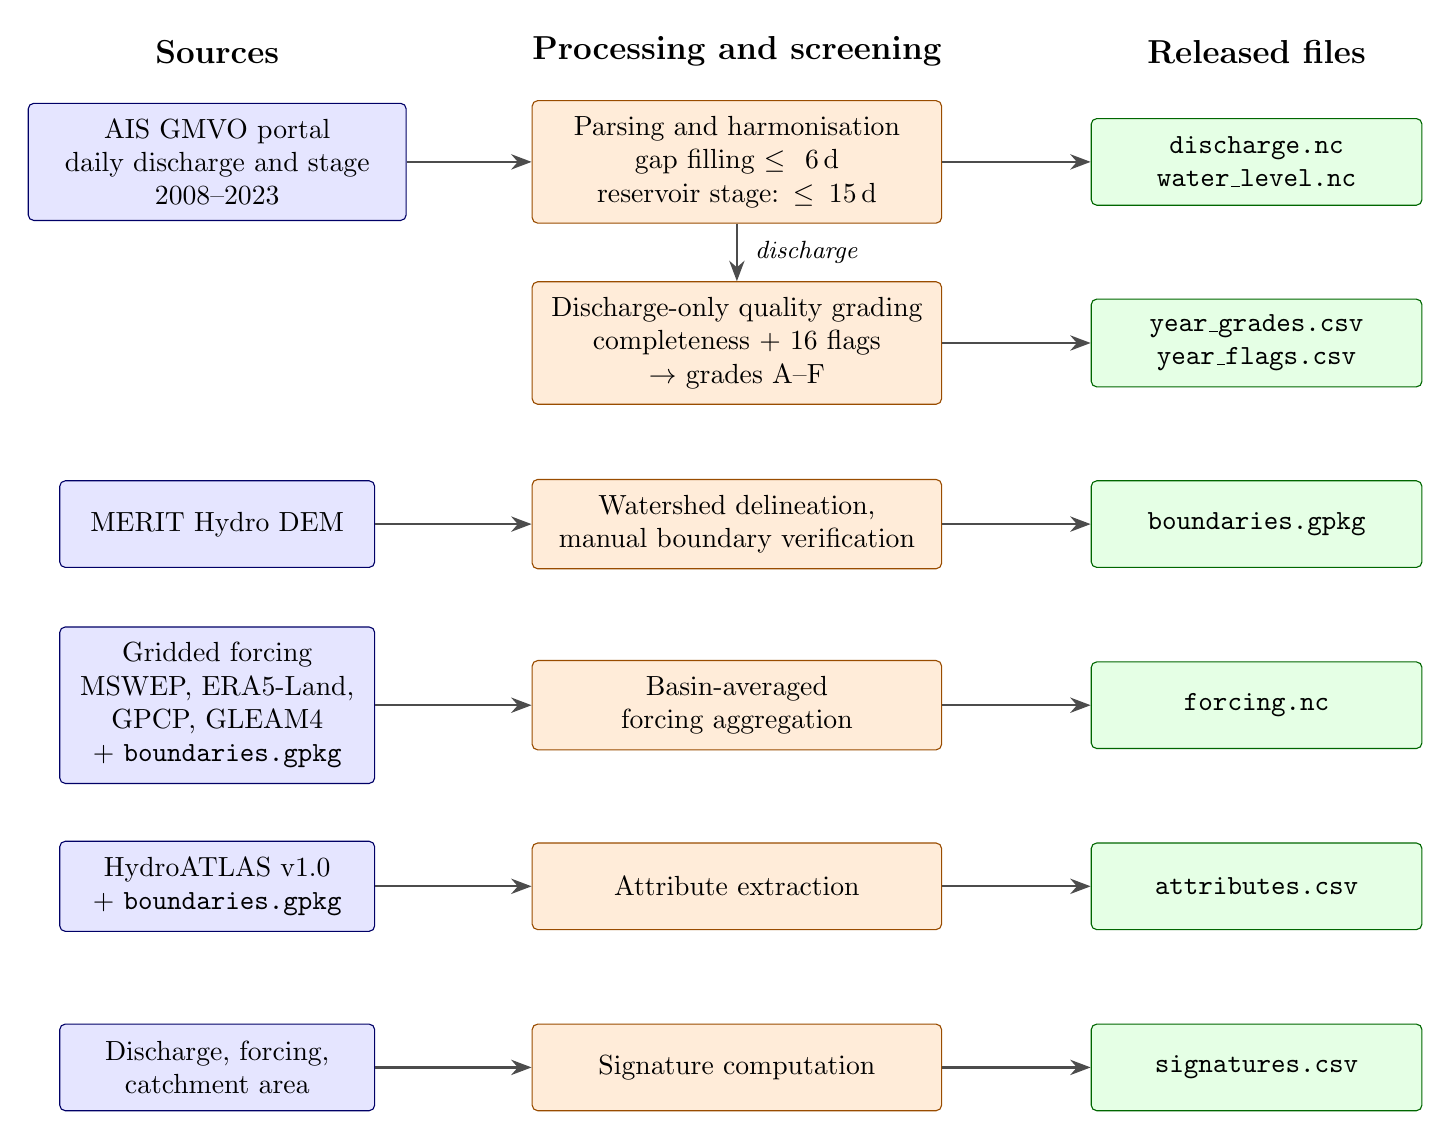
\begin{tikzpicture}[
    font=\normalsize,
    box/.style={draw, rounded corners=2pt, align=center, minimum height=11mm, inner sep=2mm},
    src/.style={box, fill=blue!10, draw=blue!40!black, text width=36mm},
    proc/.style={box, fill=orange!15, draw=orange!60!black, text width=48mm},
    outfile/.style={box, fill=green!10, draw=green!40!black, text width=38mm},
    flow/.style={-{Stealth[length=2.6mm]}, thick, draw=black!70},
  ]

  % Column x-positions and row y-positions (row-aligned: horizontal arrows only)
  \def\xsrc{0}    \def\xproc{6.6}  \def\xout{13.2}

  % Row 1 — discharge and stage
  \node[src, text width=44mm] (s1) at (\xsrc,0) {AIS GMVO portal\\ daily discharge and stage\\ 2008--2023};
  \node[proc] (p1) at (\xproc,0) {Parsing and harmonisation\\ gap filling $\leq 6$\,d\\ reservoir stage: $\leq 15$\,d};
  \node[outfile]  (o1) at (\xout,0)  {\texttt{discharge.nc}\\ \texttt{water\_level.nc}};

  % Row 2 — quality grading (fed by row 1)
  \node[proc] (p2) at (\xproc,-2.3) {Discharge-only quality grading\\ completeness + 16 flags\\ $\rightarrow$ grades A--F};
  \node[outfile]  (o2) at (\xout,-2.3)  {\texttt{year\_grades.csv}\\ \texttt{year\_flags.csv}};

  % Row 3 — delineation
  \node[src]  (s3) at (\xsrc,-4.6)  {MERIT Hydro DEM};
  \node[proc] (p3) at (\xproc,-4.6) {Watershed delineation,\\ manual boundary verification};
  \node[outfile]  (o3) at (\xout,-4.6)  {\texttt{boundaries.gpkg}};

  % Row 4 — boundaries define the basin aggregation domain
  \node[src]  (s4) at (\xsrc,-6.9)  {Gridded forcing\\ MSWEP, ERA5-Land,\\ GPCP, GLEAM4\\ + \texttt{boundaries.gpkg}};
  \node[proc] (p4) at (\xproc,-6.9) {Basin-averaged\\ forcing aggregation};
  \node[outfile]  (o4) at (\xout,-6.9)  {\texttt{forcing.nc}};

  % Row 5 — boundaries also define attribute extraction
  \node[src]  (s5) at (\xsrc,-9.2)  {HydroATLAS v1.0\\ + \texttt{boundaries.gpkg}};
  \node[proc] (p5) at (\xproc,-9.2) {Attribute extraction};
  \node[outfile]  (o5) at (\xout,-9.2)  {\texttt{attributes.csv}};

  % Row 6 — all three signature inputs are explicit
  \node[src]  (s6) at (\xsrc,-11.5)  {Discharge, forcing,\\ catchment area};
  \node[proc] (p6) at (\xproc,-11.5) {Signature computation};
  \node[outfile]  (o6) at (\xout,-11.5)  {\texttt{signatures.csv}};

  % Column headers
  \node[font=\large\bfseries] at (\xsrc,1.4)  {Sources};
  \node[font=\large\bfseries] at (\xproc,1.4) {Processing and screening};
  \node[font=\large\bfseries] at (\xout,1.4)  {Released files};

  % Horizontal flows (row-aligned, no crossings)
  \foreach \r in {1,3,4,5,6} \draw[flow] (s\r) -- (p\r);
  \foreach \r in {1,2,3,4,5,6} \draw[flow] (p\r) -- (o\r);

  % Vertical flows inside the processing column
  \draw[flow] (p1) -- (p2) node[midway, right=1mm, font=\small\itshape] {discharge};

\end{tikzpicture}
\end{document}
